\documentclass[11pt, a4paper]{article}
\usepackage{pdfpages}
\usepackage{parallel}
\usepackage[T2A]{fontenc}
\usepackage{ucs}
\usepackage[utf8x]{inputenc}
\usepackage[polish,english,russian]{babel}
\usepackage{hyperref}
\usepackage{rotating}
\usepackage[inner=2cm,top=1.8cm,outer=2cm,bottom=2.3cm,nohead]{geometry}
\usepackage{listings}
\usepackage{graphicx}
\usepackage{wrapfig}
\usepackage{longtable}
\usepackage{indentfirst}
\usepackage{array}
\usepackage{tikzsymbols}
\usepackage{soul}
\usepackage[ruled,vlined]{algorithm2e}
%\counterwithout{figure}{section} 

\usepackage{url}
\makeatletter
\g@addto@macro{\UrlBreaks}{\UrlOrds}
\makeatother

\newcolumntype{P}[1]{>{\raggedright\arraybackslash}p{#1}}
\frenchspacing
\usepackage{fixltx2e} %text sub- and superscripts
\usepackage{icomma} % коскі ў матэматычным рэжыме
\PreloadUnicodePage{4}

\newcommand{\longpage}{\enlargethispage{\baselineskip}}
\newcommand{\shortpage}{\enlargethispage{-\baselineskip}}

\def\switchlang#1{\expandafter\csname switchlang#1\endcsname}
\def\switchlangbe{
\let\saverefname=\refname%
\def\refname{Літаратура}%
\def\figurename{Іл.}%
}
\def\switchlangen{
\let\saverefname=\refname%
\def\refname{References}%
\def\figurename{Fig.}%
}
\def\switchlangru{
\let\saverefname=\refname%
\let\savefigurename=\figurename%
\def\refname{Литература}%
\def\figurename{Рис.}%
}

\hyphenation{admi-ni-stra-tive}
\hyphenation{ex-pe-ri-ence}
\hyphenation{fle-xi-bi-li-ty}
\hyphenation{Py-thon}
\hyphenation{ma-the-ma-ti-cal}
\hyphenation{re-ported}
\hyphenation{imp-le-menta-tions}
\hyphenation{pro-vides}
\hyphenation{en-gi-neering}
\hyphenation{com-pa-ti-bi-li-ty}
\hyphenation{im-pos-sible}
\hyphenation{desk-top}
\hyphenation{elec-tro-nic}
\hyphenation{com-pa-ny}
\hyphenation{de-ve-lop-ment}
\hyphenation{de-ve-loping}
\hyphenation{de-ve-lop}
\hyphenation{da-ta-ba-se}
\hyphenation{plat-forms}
\hyphenation{or-ga-ni-za-tion}
\hyphenation{pro-gramming}
\hyphenation{in-stru-ments}
\hyphenation{Li-nux}
\hyphenation{sour-ce}
\hyphenation{en-vi-ron-ment}
\hyphenation{Te-le-pathy}
\hyphenation{Li-nux-ov-ka}
\hyphenation{Open-BSD}
\hyphenation{Free-BSD}
\hyphenation{men-ti-on-ed}
\hyphenation{app-li-ca-tion}

\def\progref!#1!{\texttt{#1}}
\renewcommand{\arraystretch}{2} %Іначай формулы ў матрыцы зліпаюцца з лініямі
\usepackage{array}

\def\interview #1 (#2), #3, #4, #5\par{

\section[#1, #3, #4]{#1 -- #3, #4}
\def\qname{LVEE}
\def\aname{#1}
\def\q ##1\par{{\noindent \bf \qname: ##1 }\par}
\def\a{{\noindent \bf \aname: } \def\qname{L}\def\aname{#2}}
}

\def\interview* #1 (#2), #3, #4, #5\par{

\section*{#1\\{\small\rm #3, #4. #5}}
\ifx\ParallelWhichBox\undefined%
    \addcontentsline{toc}{section}{#1, #3, #4}%
\else%
\ifnum\ParallelWhichBox=0%
    \addcontentsline{toc}{section}{#1, #3, #4}%
\fi\fi%

\def\qname{LVEE}
\def\aname{#1}
\def\q ##1\par{{\noindent \bf \qname: ##1 }\par}
\def\a{{\noindent \bf \aname: } \def\qname{L}\def\aname{#2}}
}

\newcommand{\interviewfooter}[1]{
\vskip 1em
\noindent \textit{#1}
}

\switchlang{ru}
\begin{document}

\title{1998 "--- Трекбол Logitech TrackMan Marble FX}
\date{}
\maketitle
\selectlanguage{russian}
Безусловно, основной отличительной особенностью трекбола Trackman Marble FX (рис. \ref{fig:trackman}), выпущенного компанией Logitech в 1998 году, является его необычная форма, предоставляющая опору для запястья и открывающая доступ к шару сразу с обеих сторон корпуса. По задумке производителя, это позволяет перемещать шар либо одним пальцем, либо двумя одновременно (большим и указательным) для максимальной точности малых перемещений курсора \cite{marbleBoot}.

\begin{figure}[h]
    \centering
    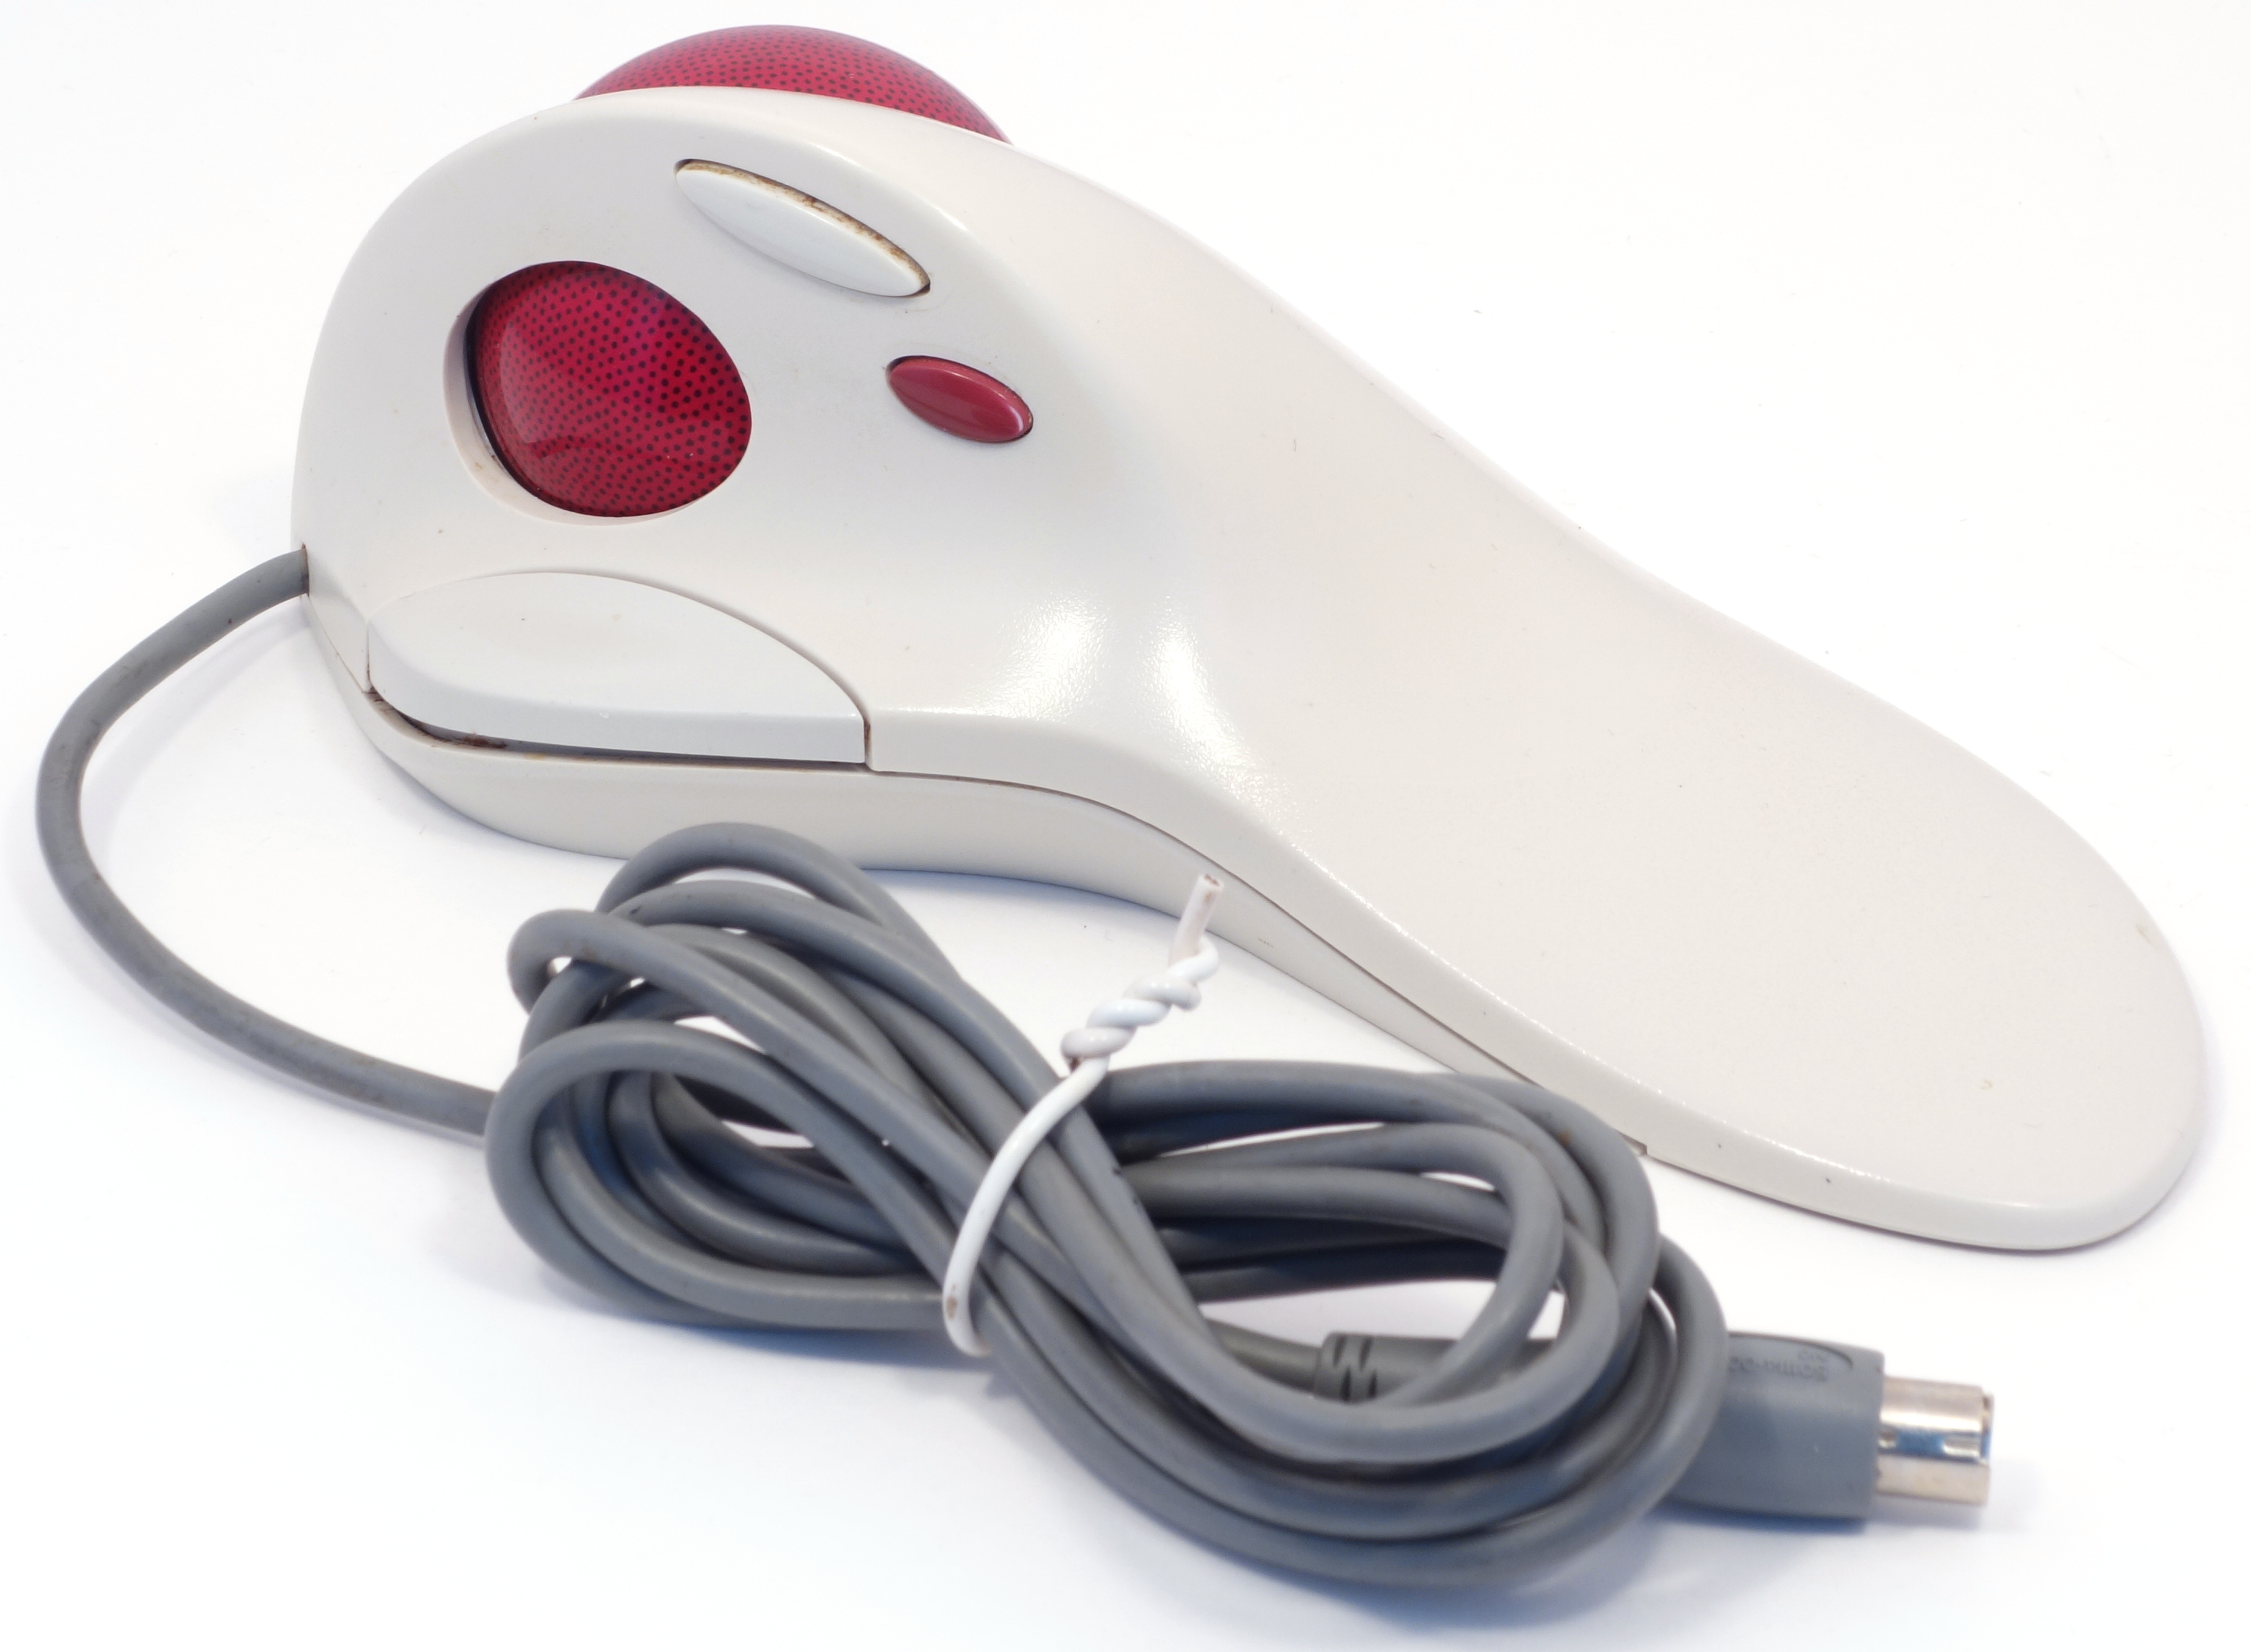
\includegraphics[scale=0.38]{1998_logitech_trackman_marble_fx/pic_30.jpg}
    \caption{Изображение Logitech TrackMan Marble FX}
    \label{fig:trackman}
\end{figure}

Сложная форма, наводящая на мысли о скалах, подверженных длительной работе ветра или волн, соответствует скорее стилю дизайнерских манипуляторов Луиджи Колани, чем каким-либо прежним разработкам Logitech. Трекбол получился ярким, запоминающимся, и совершенно заслуженно стал призером престижной премии <<IF Design Award>> проектной организации «iF International Forum Design GmbH» \cite{award}.

\begin{figure}[h]
    \centering
    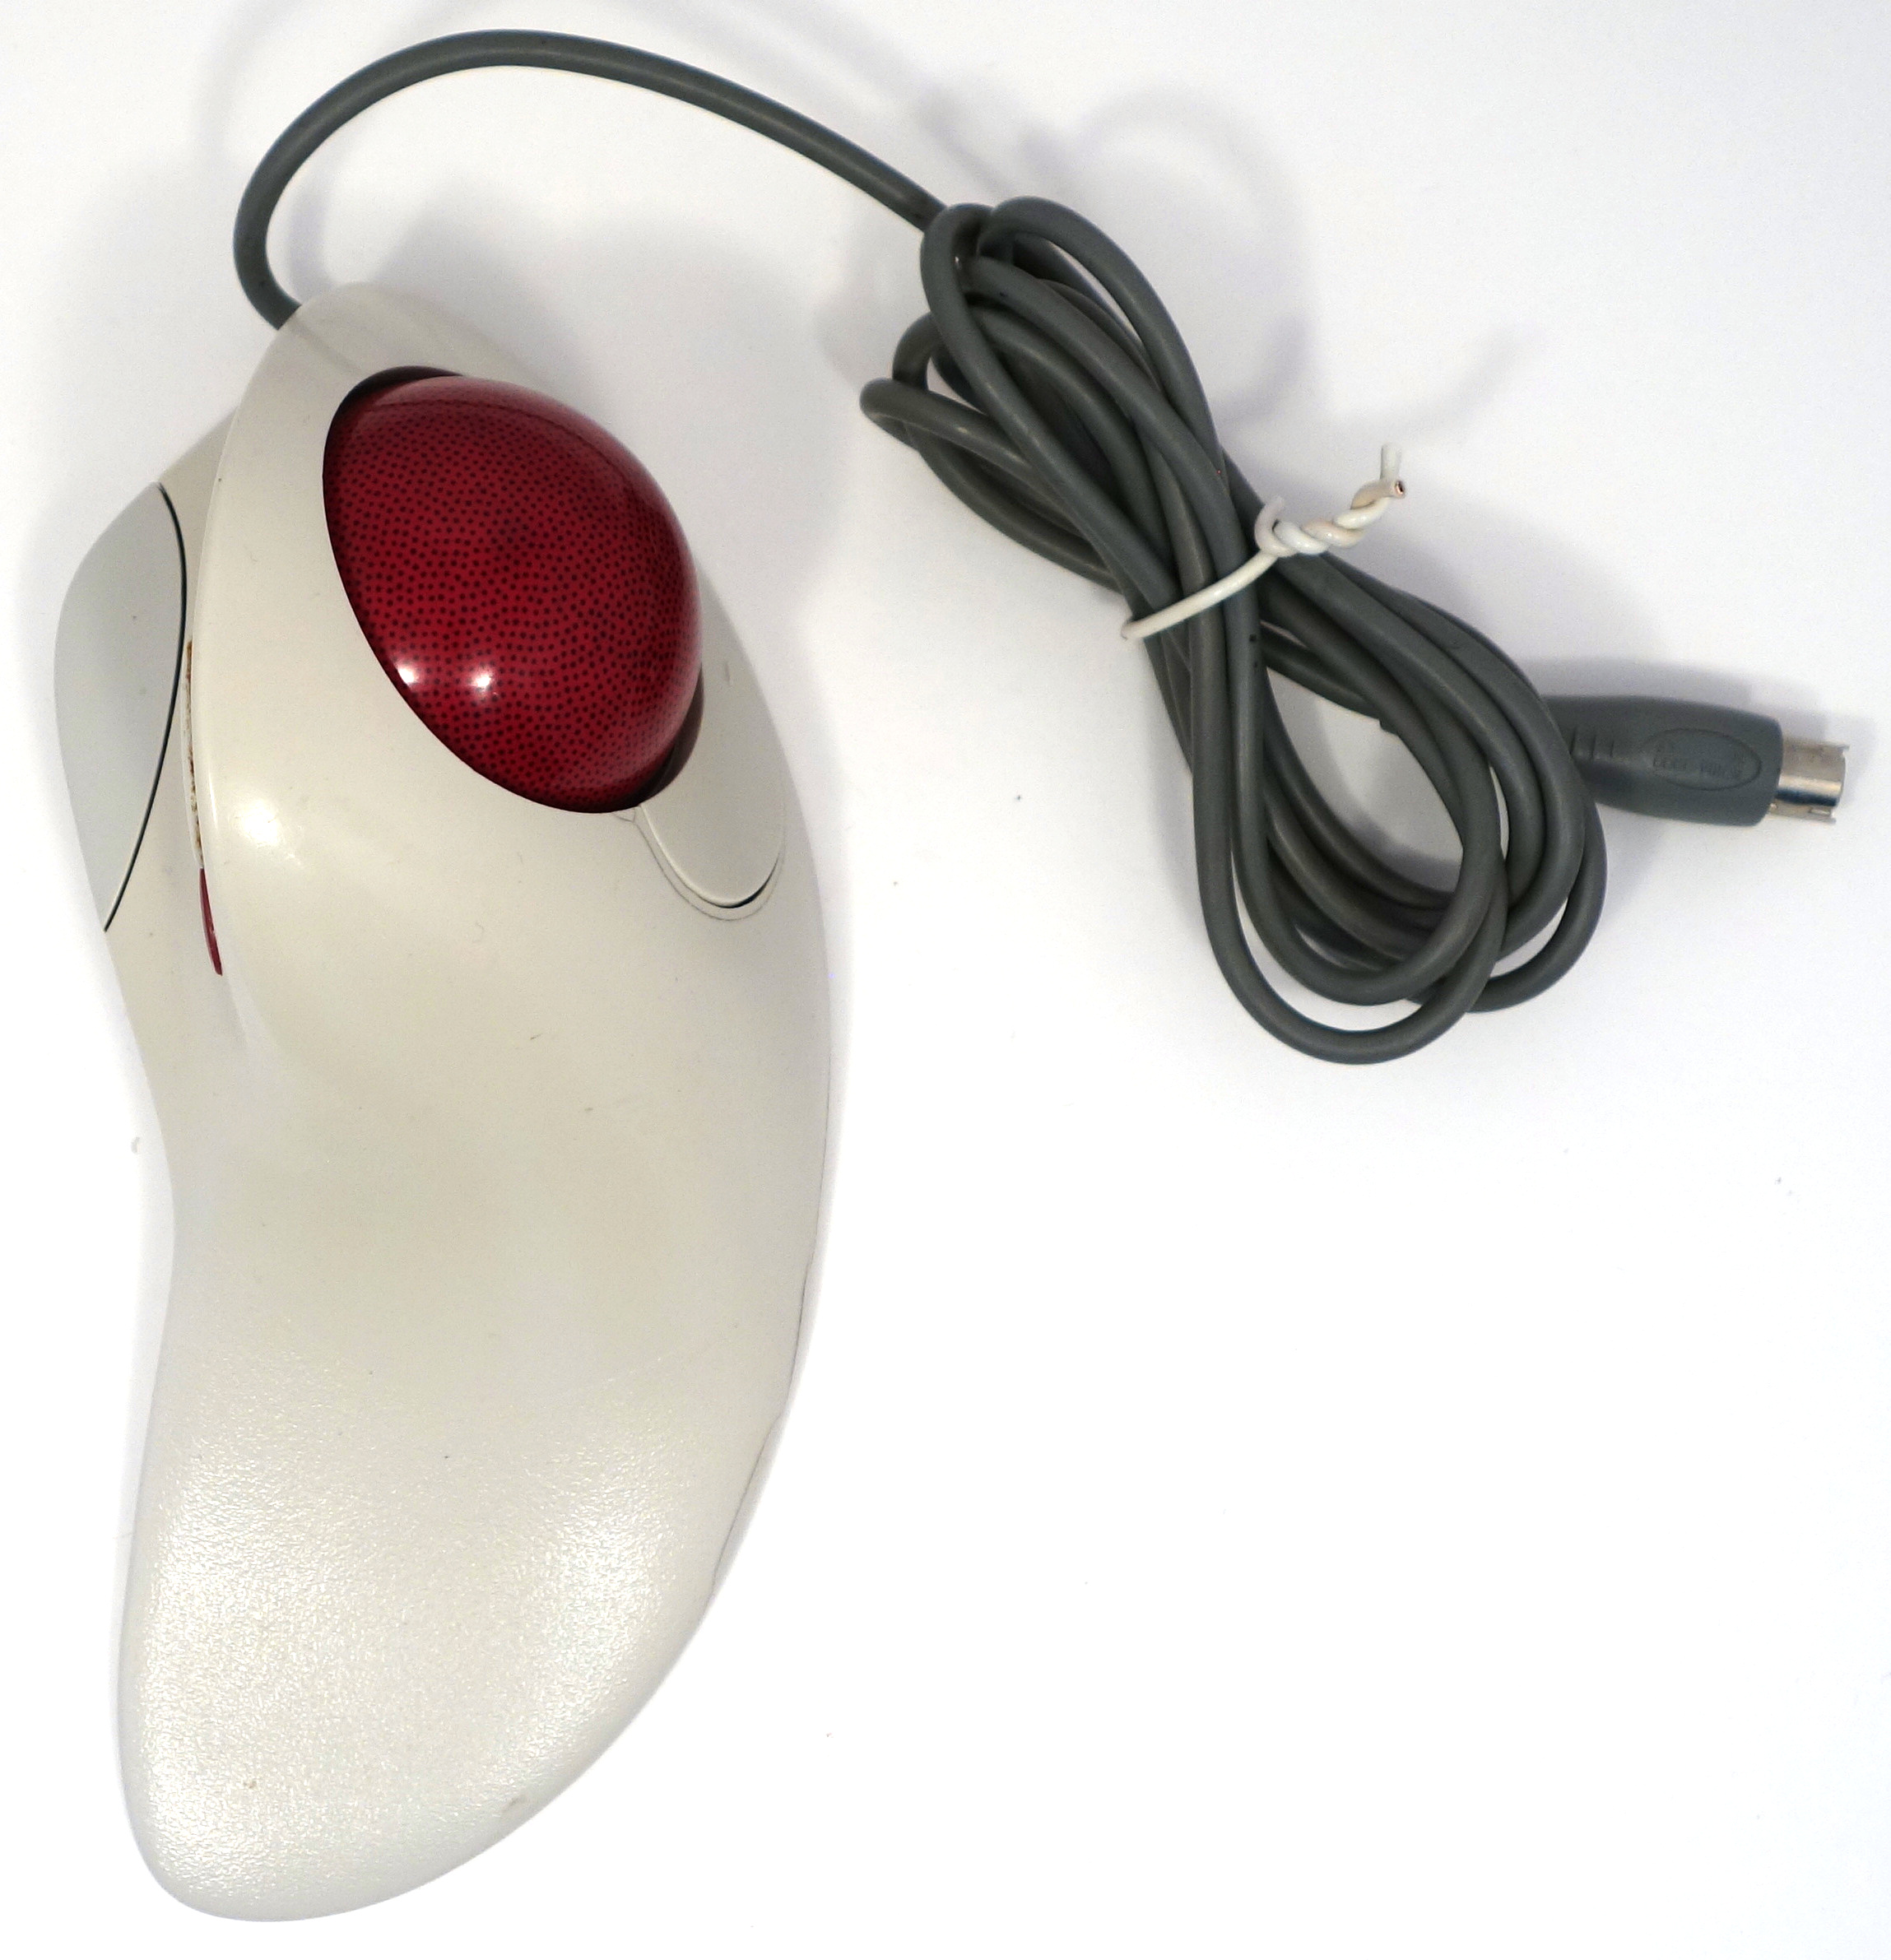
\includegraphics[scale=0.32]{1998_logitech_trackman_marble_fx/top_60.jpg}
    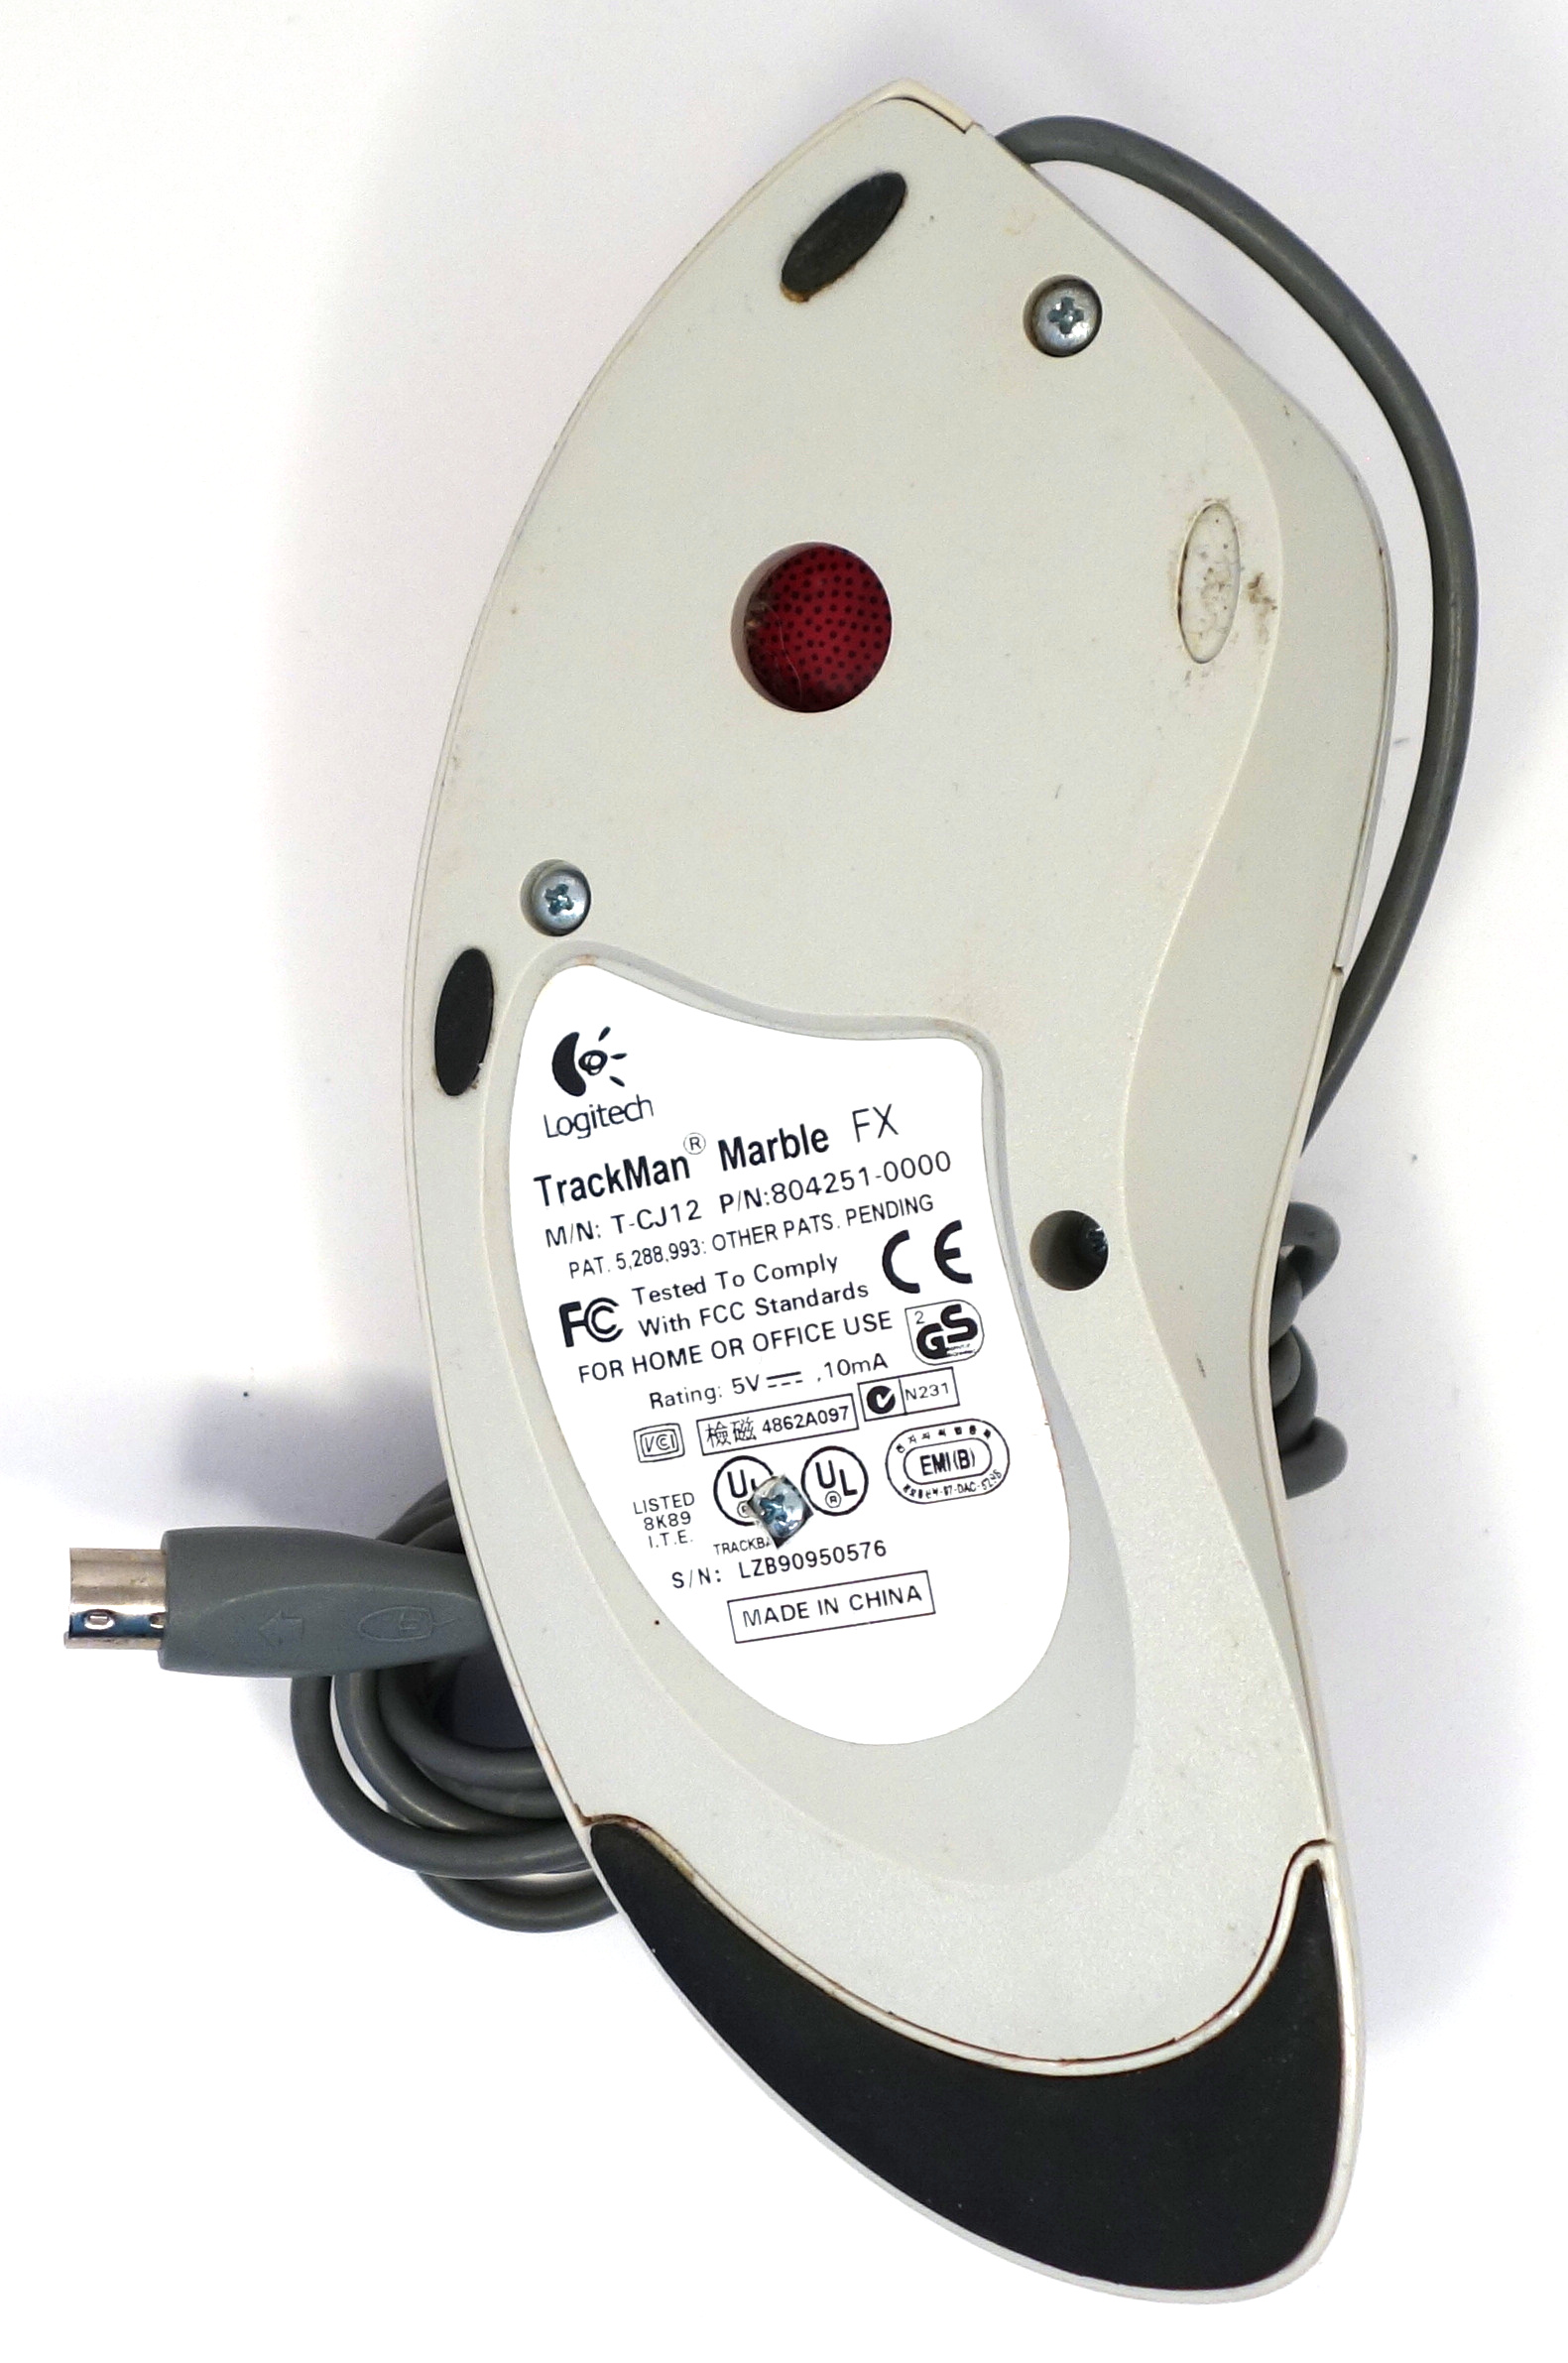
\includegraphics[scale=0.32]{1998_logitech_trackman_marble_fx/bottom_60.jpg}
    \caption{Изображение Logitech TrackMan Marble FX, вид сверху и снизу}
    \label{fig:trackmanTopAndBottom}
\end{figure}

Клавиш у TrackMan Marble FX четыре: три на левой стороне корпуса и одна на правой (рис. \ref{fig:trackmanTopAndBottom}).
Кнопки белого цвета отвечают за стандартные функции кнопок мыши, а при нажатии на красную кнопку, расположенную недалеко от шара, поставлявшийся в комплекте с трекболом драйвер переключался между режимом перемещения курсора и режимом прокрутки/масштабирования.

Регулярный узор из тёмных точек на поверхности шара вызван применением оптического датчика для считывания перемещений. Подключение к компьютеру осуществляется по интерфейсу PS/2.

\begin{figure}[h]
    \centering
    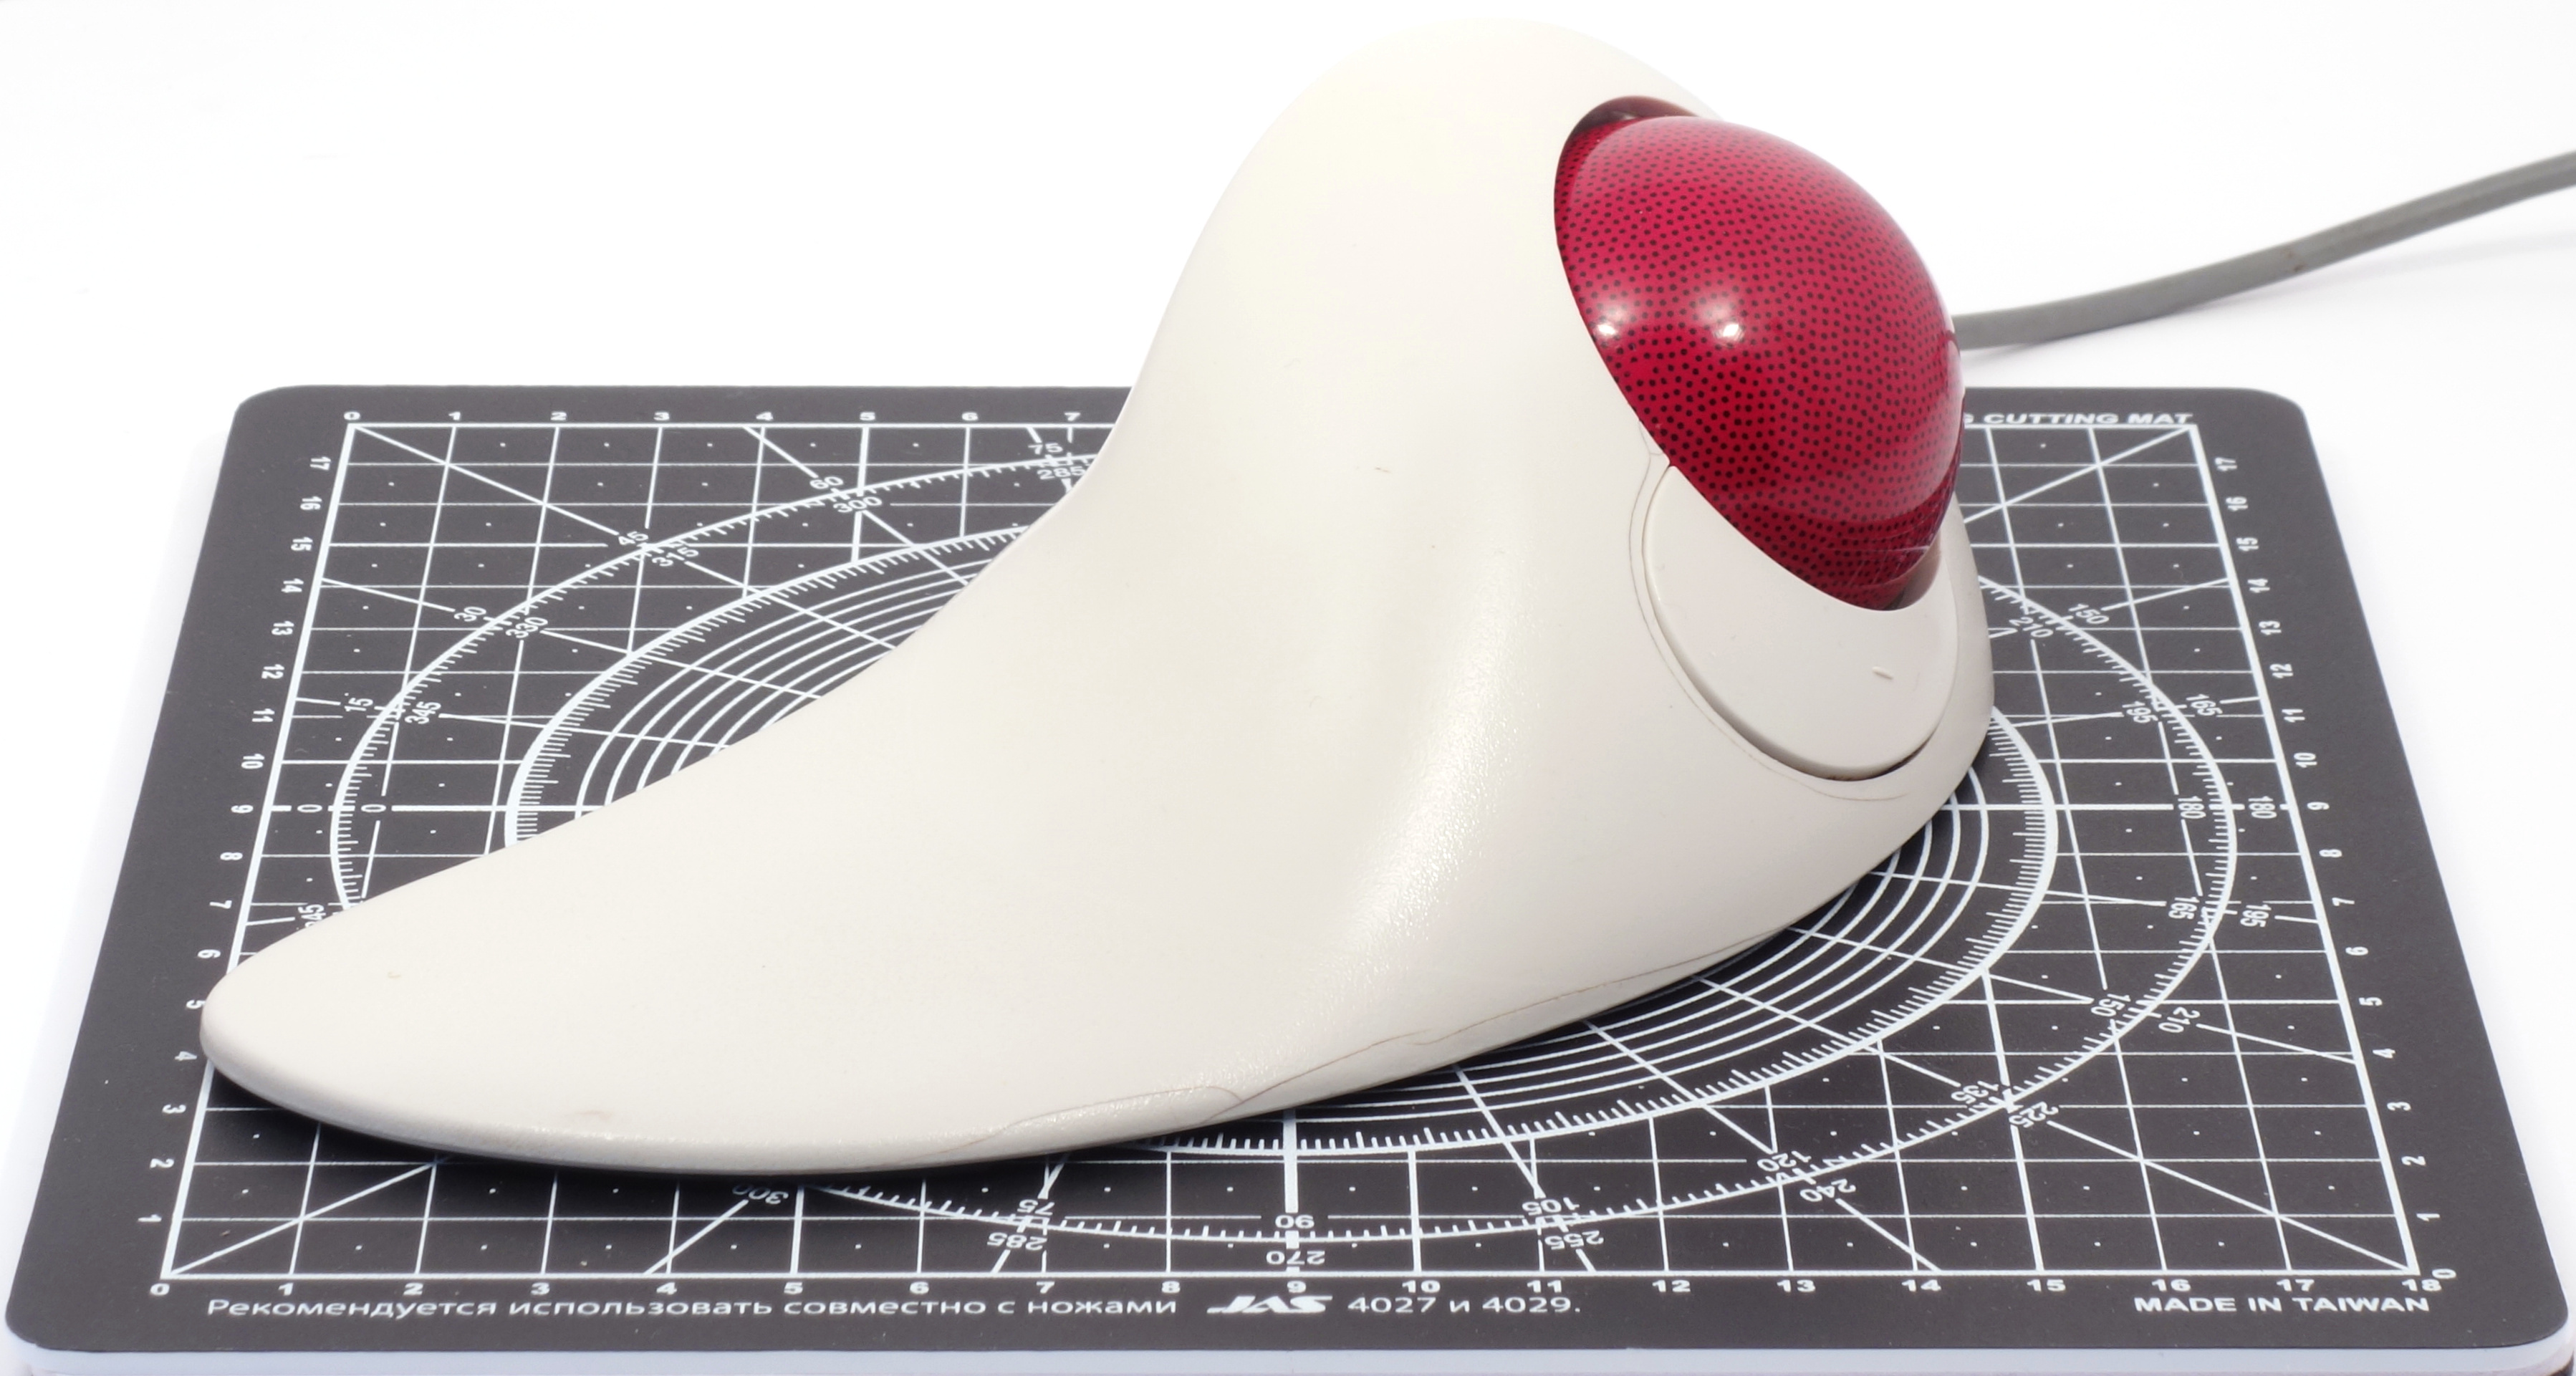
\includegraphics[scale=0.4]{1998_logitech_trackman_marble_fx/size_30.jpg}
    \caption{Изображение Logitech TrackMan Marble FX на размерном коврике с шагом сетки 1 см}
    \label{fig:trackmanSize}
\end{figure}

TrackMan Marble FX имеет крупные размеры и шар б\'{о}льшего диаметра, чем у предыдущих трекболов Logitech (рис. \ref{fig:trackmanSize}). Трекбол асимметричен и предназначен для использования исключительно правой рукой, а наклон и изгибы корпуса нацелены на то, чтобы запястье руки пользователя находилось в максимально естественном положении (рис. \ref{fig:trackmanHand}).

\begin{figure}[h]
    \centering
    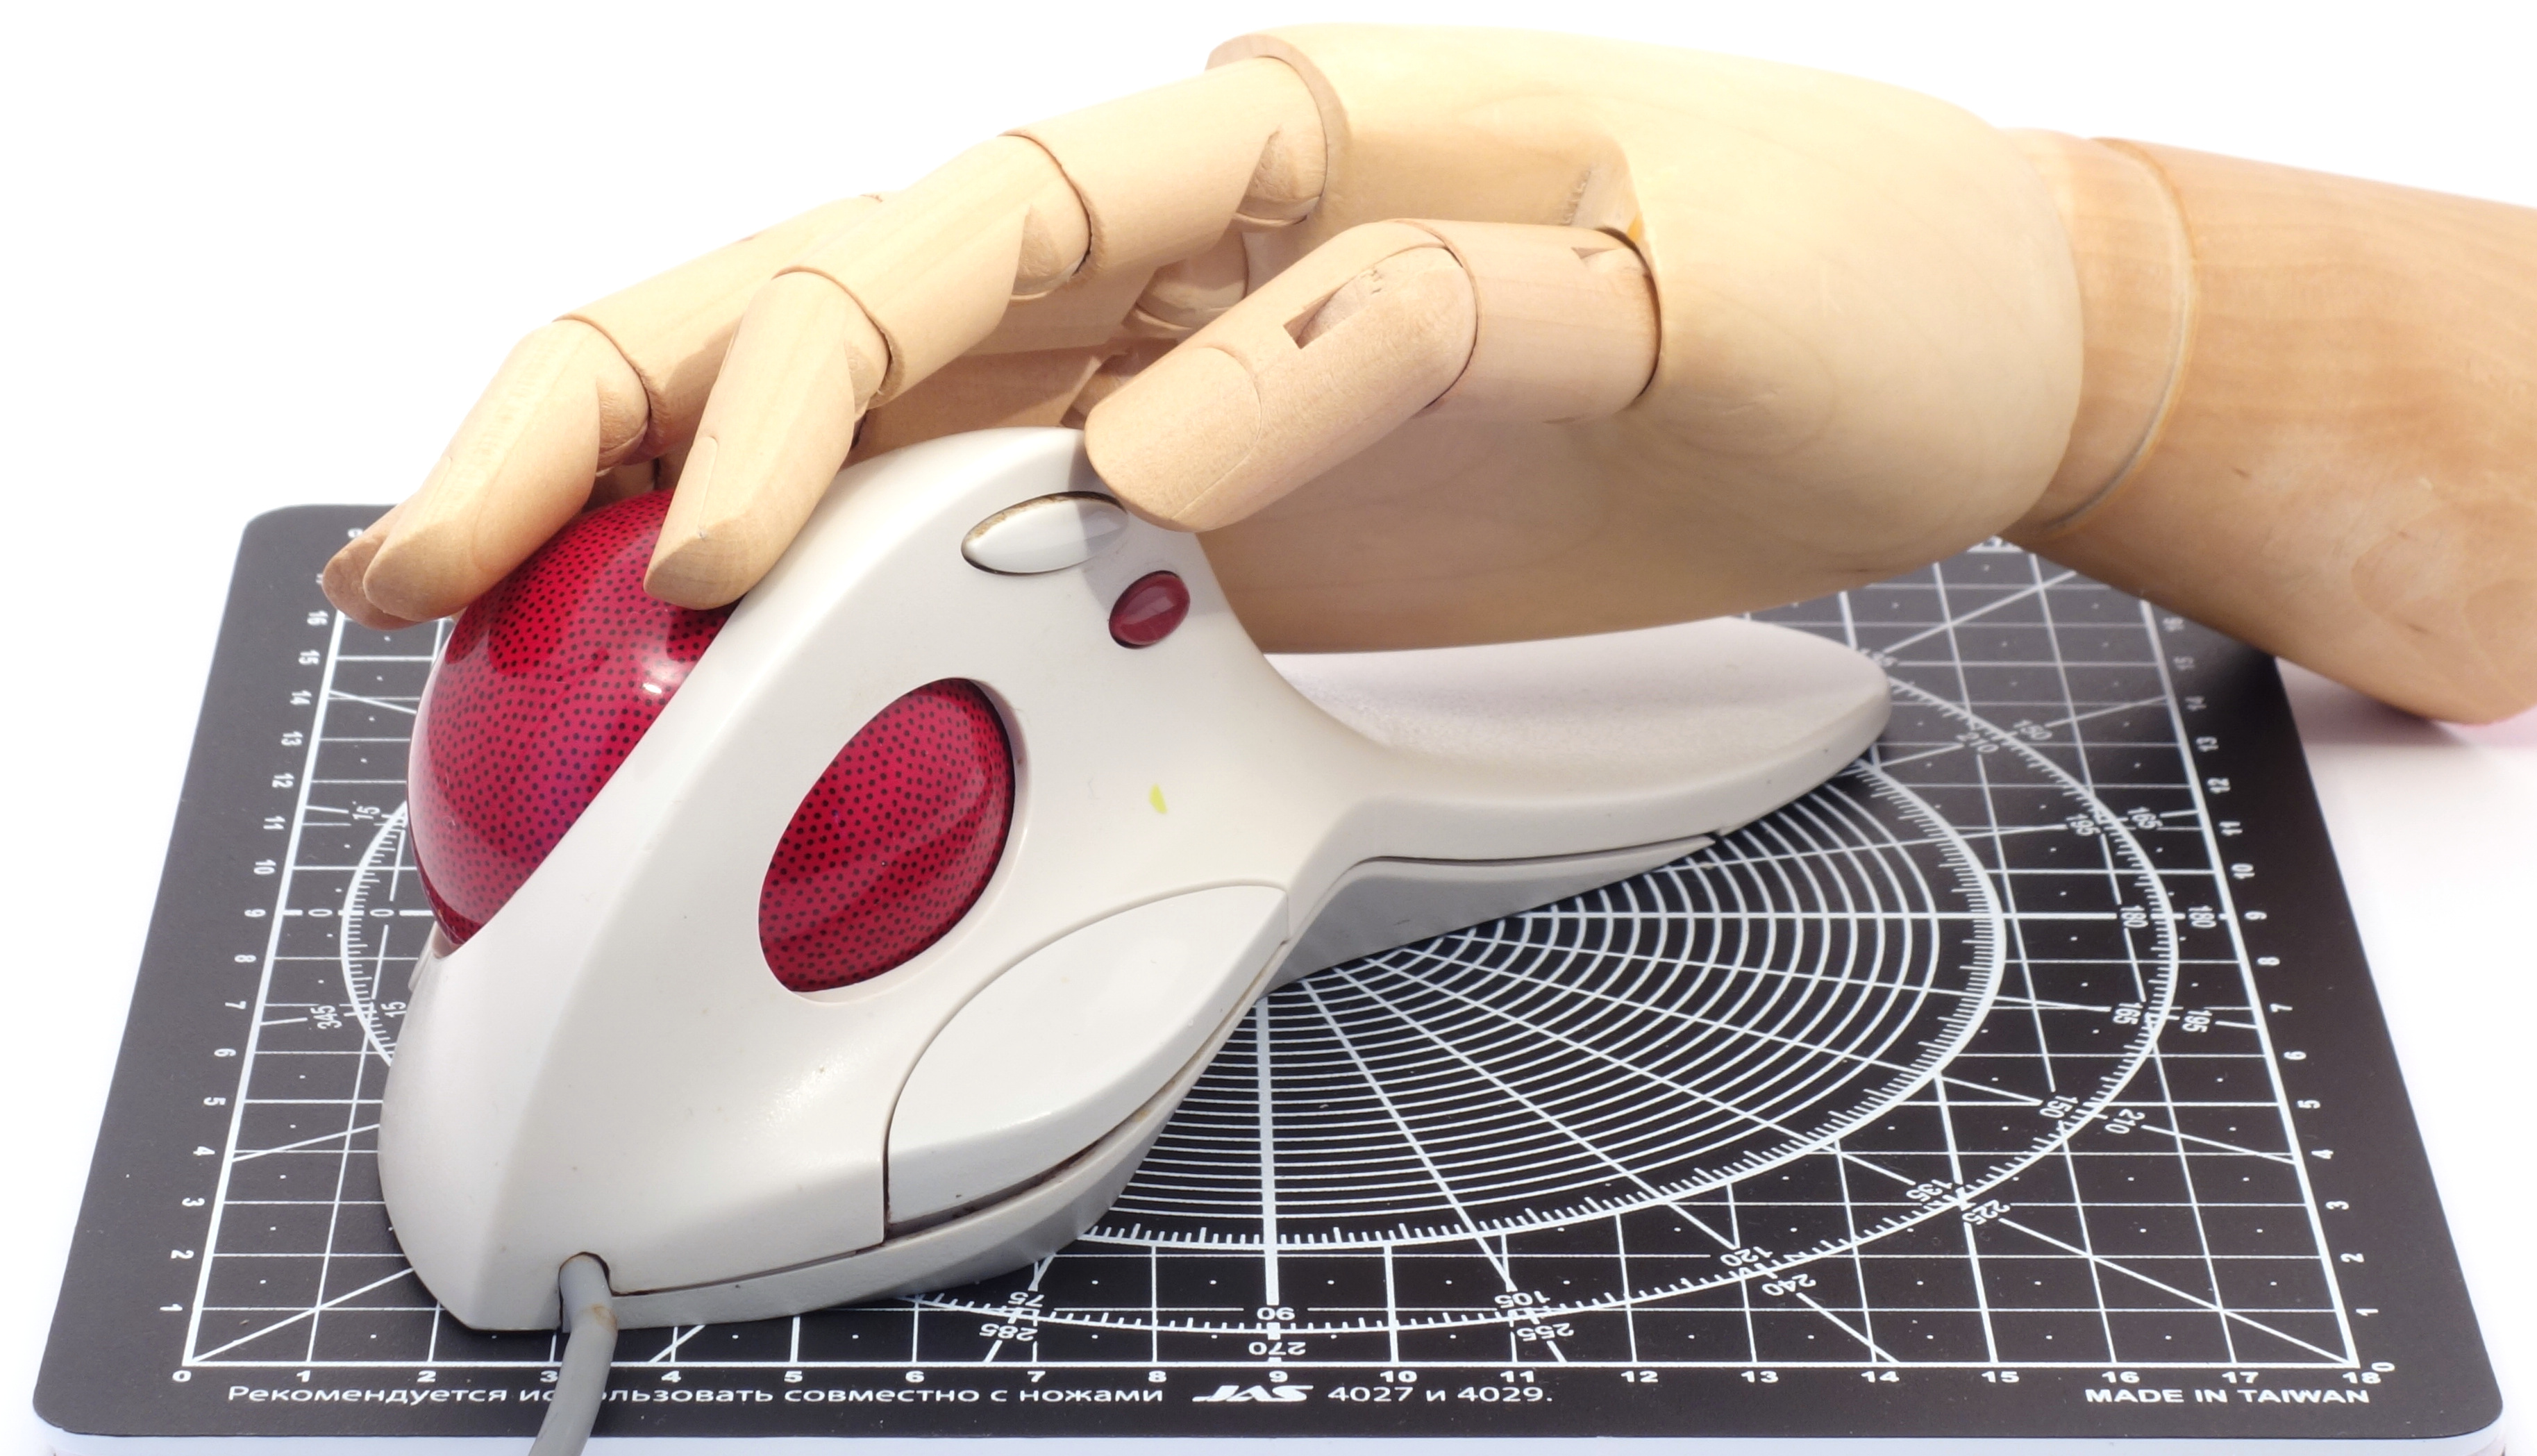
\includegraphics[scale=0.6]{1998_logitech_trackman_marble_fx/hand_30.jpg}
    \caption{Изображение Logitech TrackMan Marble FX с моделью руки человека}
    \label{fig:trackmanHand}
\end{figure}

В статьях, опубликованных в ZDNET \cite{zdnet} и в журнале Computer Gaming World \cite{gaming} отмечается, что TrackMan Marble FX достаточно удобен в использовании, но отверстие в корпусе, задуманное чтобы шар можно было перемещать пальцами с двух сторон, на практике не очень подходит для этой цели из-за своего малого размера (скорее, оно несет эстетическую функцию,а также облегчает извлечение шара из корпуса для чистки). Кроме того, часть корпуса, являющаяся подставкой под запястье, вызывала смешанную реакцию у некоторых пользователей, которые предпочли бы большую гибкость за счет использования в этой роли съемного аксессуара.

Разбор трекбола (рис. \ref{fig:trackmanInside}) показывает конструкцию, являющуюся аналогом оптической мыши, считывавшей изменения яркости с помощью специального коврика с нанесенной на нём сеткой (роль коврика играет рисунок на шаре).

\begin{figure}[h]
    \centering
    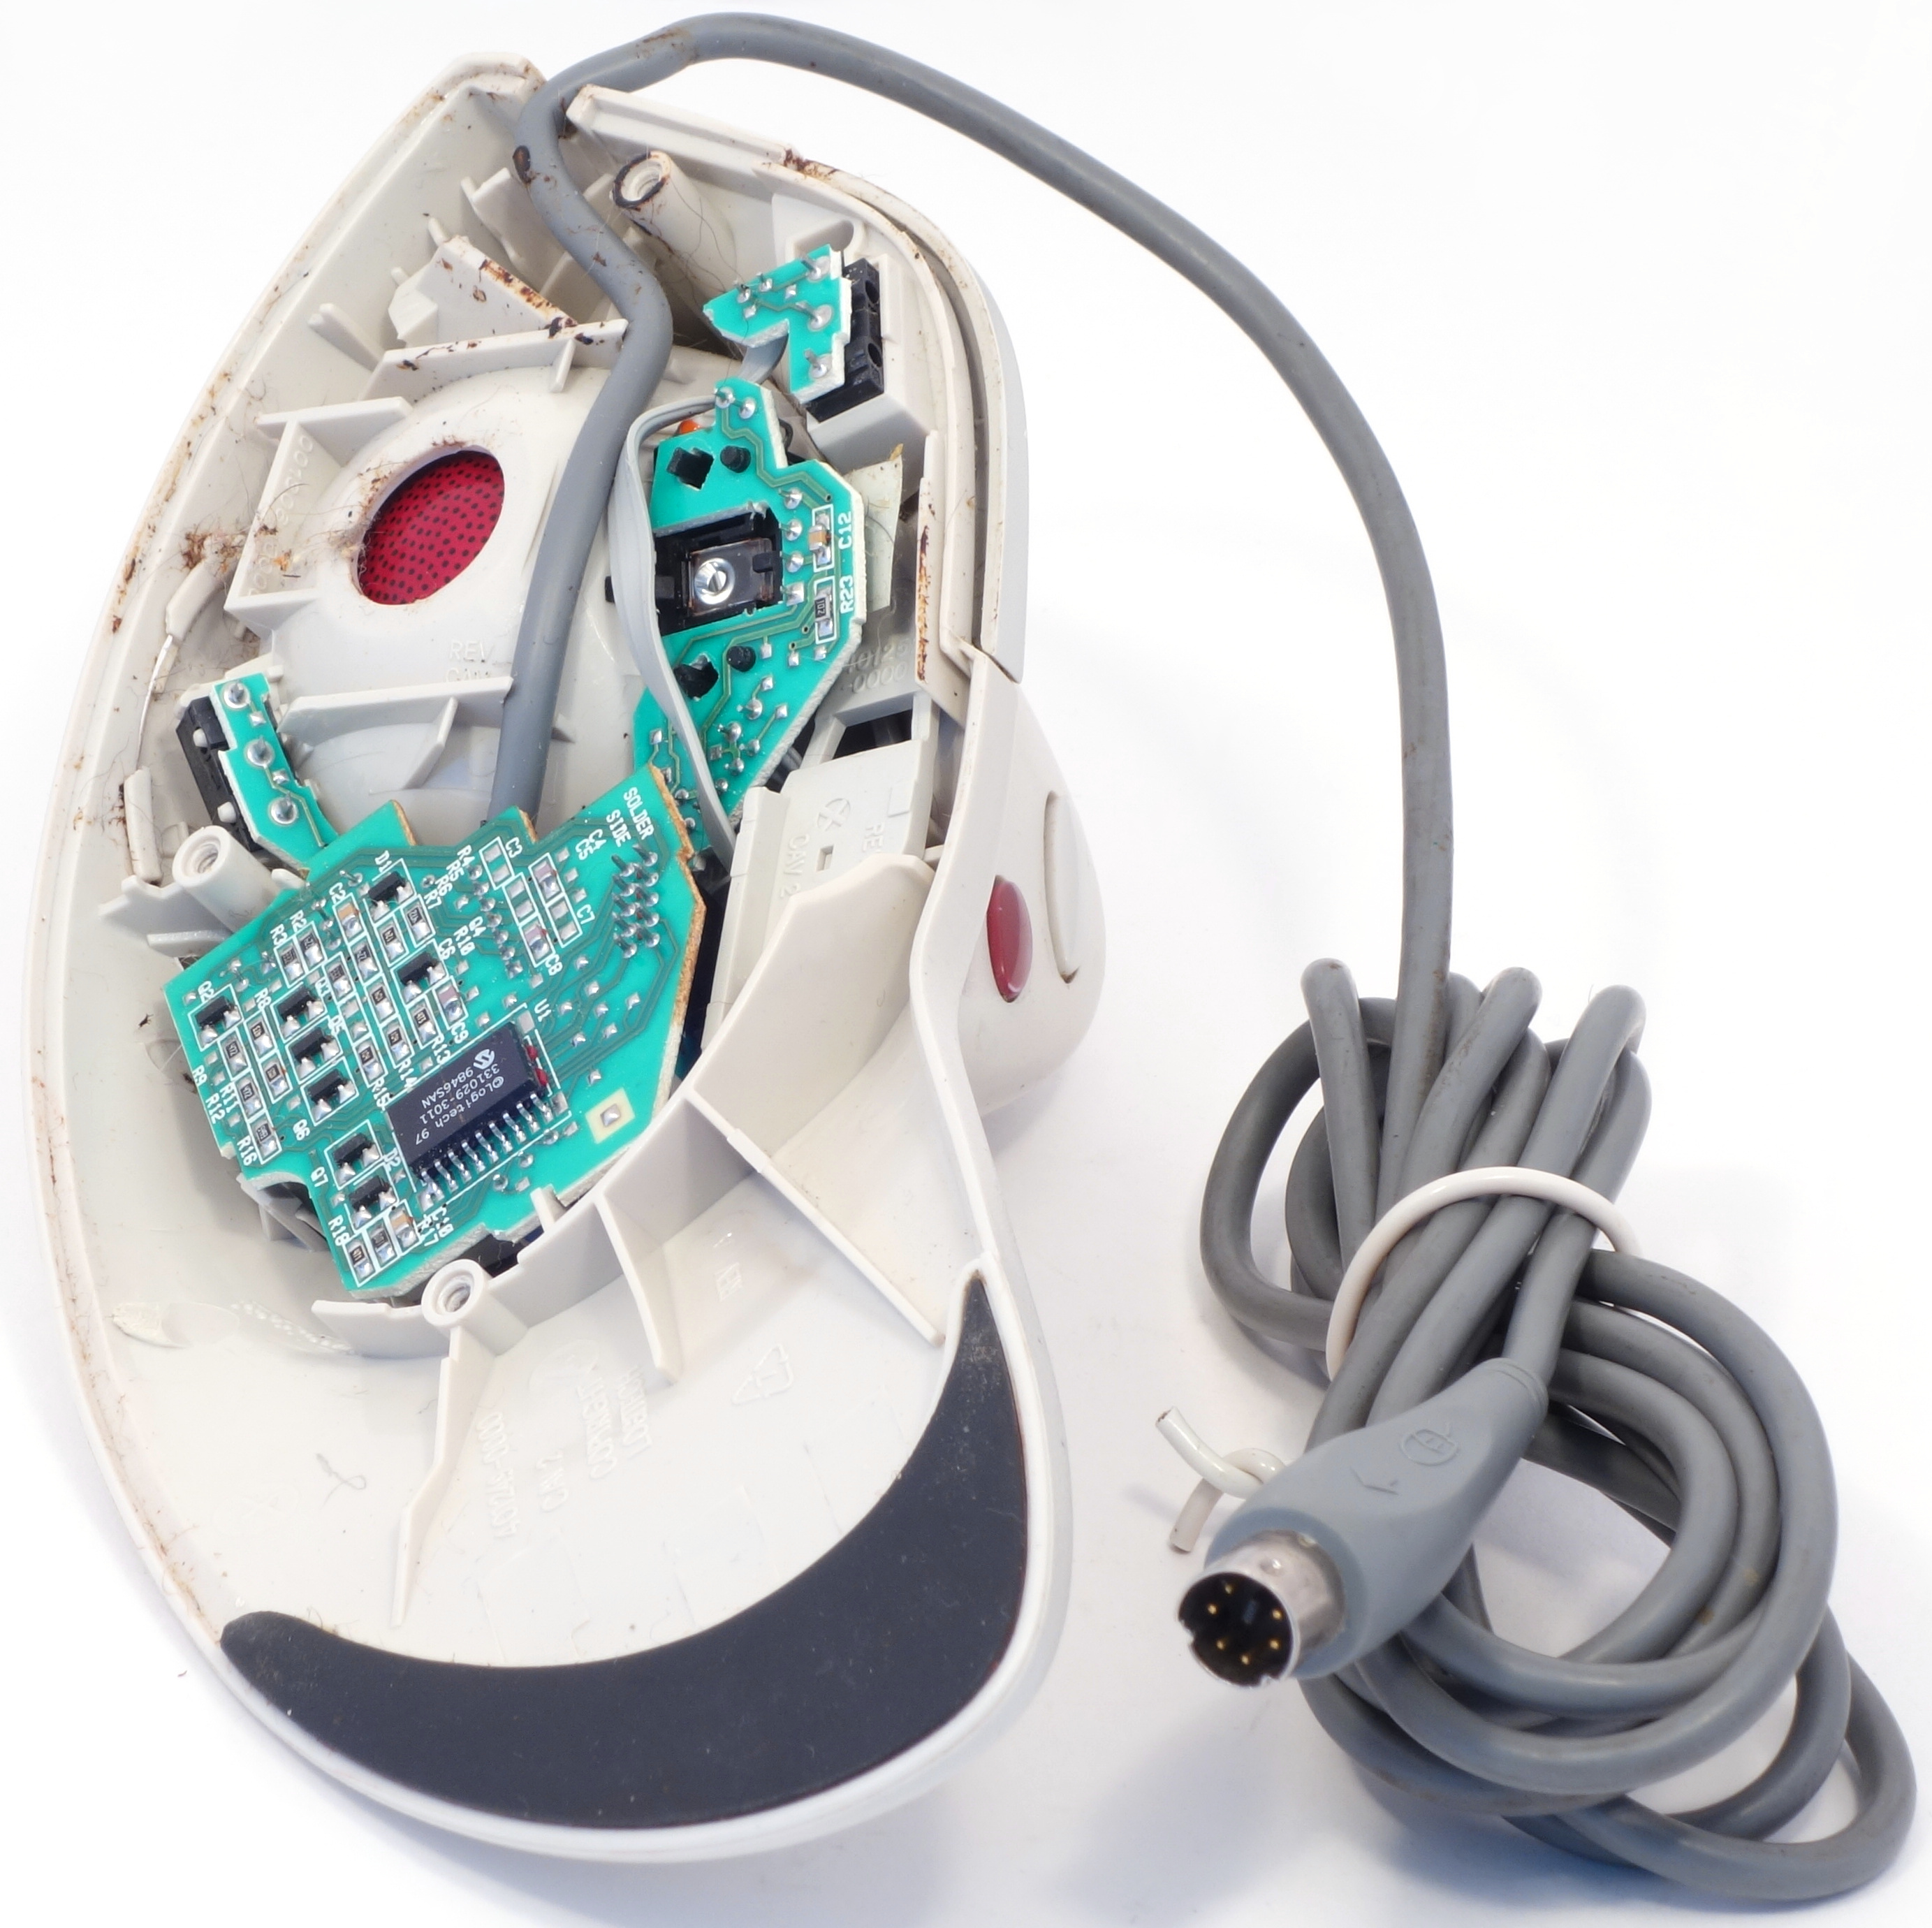
\includegraphics[scale=0.6]{1998_logitech_trackman_marble_fx/inside_30.jpg}
    \caption{Изображение Logitech TrackMan Marble FX изнутри}
    \label{fig:trackmanInside}
\end{figure}

\begin{thebibliography}{9}
\bibitem{marbleBoot} Pure lust. High-tech toys and tools with the right stuff. // Boot Magazine: Issue 20 - April 1998. -- p. 18. \url{https://archive.org/details/boot-magazine-issue20-pc-notebook-autopsy-apr-1998/page/n19/mode/2up}
\bibitem{gaming} Case L. Revew - Logitech Trackman Marble/FX. Absolutely Marble-ous. // Computer Gaming World: Issue 168 - July 1998. -- p. 127.  \url{https://archive.org/details/Computer_Gaming_World_Issue_168/page/n129/mode/2up}
\bibitem {zdnet} Watson J.A. Trackballs that I have known and loved: A history in hardware. - ZDNET, March 16, 2017. \url{https://www.zdnet.com/article/trackballs-that-i-have-known-and-loved-a-history-in-hardware/}
\bibitem {award} IF Design - TrackMan Marble FX \url{https://ifdesign.com/en/winner-ranking/project/trackman-marble-fx/16939}
\end{thebibliography}

\end{document}
